\documentclass[11pt,a4paper]{report}

\usepackage[french]{babel}
\usepackage[utf8]{inputenc}
\usepackage[T1]{fontenc}
\usepackage[a4paper,margin=2.5cm]{geometry}
\usepackage{graphicx}
\usepackage{booktabs}
\usepackage{longtable}
\usepackage{xcolor}
\usepackage{hyperref}
\usepackage{amsmath}
\usepackage{amssymb}
\usepackage{enumitem}

\newcommand{\todonote}[1]{\textcolor{red}{\textbf{[À COMPLÉTER : #1]}}}

\title{Segmentation automatique et interprétable de structures anatomiques \\
sur IRM dynamique du défilé cervico-thoracique \\
\large Baseline FLASH vs RSSFP -- méthodologie littérature-first \\
\large Rapport de suivi de thèse}
\author{Yasmine Ben Abdelkader}
\date{Document vivant --- dernière mise à jour : \today}

\hypersetup{colorlinks=true, linkcolor=blue, urlcolor=blue, citecolor=blue}

\begin{document}
\maketitle
\tableofcontents

\chapter{Contexte et objectifs}
\label{chap:contexte}

\section{Problématique clinique}

Le syndrome de défilé cervico-thoracique (\emph{Thoracic Outlet Syndrome}, TOS) est une pathologie
liée à la compression de structures neurovasculaires au niveau du défilé cervico-thoracique lors de
certains mouvements du bras. Le diagnostic s'appuie sur une IRM \textbf{dynamique} : une séquence
d'environ 300 images acquises pendant le mouvement du bras, jouant le rôle d'une vidéo, mais stockée
physiquement comme des fichiers DICOM individuels (un fichier par image, sans tag DICOM natif de
vidéo/temporalité).

\section{Objectif de la thèse}

L'objectif \textbf{n'est pas} de maximiser la performance brute d'un modèle de segmentation, mais de
comprendre \emph{comment} un modèle de deep learning arrive à ses segmentations sur ce type de données.
L'\textbf{interprétabilité / explicabilité} est la contribution centrale de la thèse ; un modèle de
segmentation performant est un moyen, pas une fin en soi.

Six structures anatomiques sont ciblées :

\begin{itemize}[nosep]
    \item \textbf{CLAV} --- clavicule
    \item \textbf{MSC} --- muscle scalène
    \item \textbf{VSC} --- veine sous-clavière
    \item \textbf{ASC} --- artère sous-clavière
    \item \textbf{K1} --- première côte
    \item \textbf{PB} --- plexus brachial
\end{itemize}

Ces six structures ont été confirmées mutuellement exclusives (pas de recouvrement inter-pixel), ce
qui oriente le choix de sortie du modèle vers un softmax multi-classe plutôt qu'un sigmoïde
multi-label.

\section{Plan de travail en six phases}

\begin{description}[style=nextline]
    \item[Phase 0 --- Préparation des données] Finalisation du nettoyage identifié en exploration
        (rééchantillonnage, normalisation des noms de segments, gestion des masques 4D/multi-couches),
        construction d'un jeu de données (image, masque) aligné et consolidé, définition d'un split
        train/val/test au niveau patient (14 patients --- attention aux fuites de données).
    \item[Phase 1 --- Modèle baseline] U-Net 2D simple (volontairement non état de l'art), entraîné
        sur les 20 images annotées par série. Dice/Hausdorff par structure comme référence de sanité,
        pas comme objectif d'optimisation.
    \item[Phase 2 --- Boîte à outils XAI] Seg-Grad-CAM (saillance par structure), MC Dropout (cartes
        d'incertitude par structure), analyse par occlusion. Validation qualitative des outils
        eux-mêmes avant d'en exploiter les résultats.
    \item[Phase 3 --- Analyse spécifique au caractère dynamique (axe original)] Cohérence temporelle
        des explications (la saillance dérive-t-elle de façon lisse d'une image à l'autre, comme
        l'anatomie réelle, ou de façon erratique ?), courbe de compression costoclaviculaire
        (distance CLAV--K1 en fonction du temps) pour localiser les images cliniquement critiques,
        corrélation entre incertitude/saillance et distance à l'image annotée la plus proche.
    \item[Phase 4 --- Ancrage clinique] Curation d'environ 10 à 15 cas représentatifs, session de
        validation qualitative avec le radiologue superviseur comparant les explications du modèle
        au raisonnement clinique.
    \item[Phase 5 --- Extension optionnelle] Entraînement d'une seconde architecture (p.\,ex.
        attention U-Net) sur le même split pour comparer le comportement d'interprétabilité à
        performance égale ; éventuellement TCAV sur des concepts cliniques, influence functions /
        leave-one-out sur les 20 images annotées.
    \item[Phase 6 --- Synthèse] Table récapitulative par structure (Dice + incertitude + qualité des
        explications + avis clinicien), rédaction finale.
\end{description}

\section{État d'avancement}

\begin{itemize}[nosep]
    \item[\checkmark] Exploration des données (EDA) --- voir chapitre~\ref{chap:exploration}
    \item[$\square$] Phase 0 --- Préparation des données
    \item[$\square$] Phase 1 --- Modèle baseline
    \item[$\square$] Phase 2 --- Boîte à outils XAI
    \item[$\square$] Phase 3 --- Analyse dynamique
    \item[$\square$] Phase 4 --- Ancrage clinique
    \item[$\square$] Phase 5 --- Extension optionnelle
    \item[$\square$] Phase 6 --- Synthèse
\end{itemize}

\chapter{Données}

\section{Organisation générale}

Les données sont stockées dans \texttt{EPAPLEX/DATA/}. Le jeu de données comprend
\textbf{14 patients} (dossiers nommés par exemple \texttt{2017-110\_01-0229-V1MR}), chacun disposant
de \textbf{4 séries} :

\begin{itemize}[nosep]
    \item \texttt{FLASH D} (droite)
    \item \texttt{FLASH G} (gauche)
    \item \texttt{RSSFP D} (droite)
    \item \texttt{RSSFP G} (gauche)
\end{itemize}

Soit 56 séries au total. Chaque série contient 20 images DICOM annotées
(\texttt{IM\_001.dcm}, \ldots, \texttt{IM\_020.dcm}) extraites de l'acquisition dynamique complète
(environ 300 images), ainsi qu'un volume prétraité \texttt{volume\_n4.npy} (correction du champ de
biais N4) --- lorsqu'il est disponible (voir \S\ref{sec:n4-manquant}).

\section{Vérité terrain}

Le fichier \texttt{Segmentation\_PB.seg.nrrd} est le labelmap multi-label de référence contenant les
6 structures cibles dans un seul volume :

\begin{center}
\begin{tabular}{cl}
\toprule
Label & Structure \\
\midrule
1 & CLAV --- clavicule \\
2 & MSC --- muscle scalène \\
3 & VSC --- veine sous-clavière \\
4 & ASC --- artère sous-clavière \\
5 & K1 --- première côte \\
6 & PB --- plexus brachial \\
\bottomrule
\end{tabular}
\end{center}

\todonote{Confirmer cette correspondance label $\to$ structure avec le directeur de thèse.}

D'autres fichiers \texttt{Segmentation\_*.seg.nrrd} (\texttt{sPB}, \texttt{Just-PB},
\texttt{CLAV\_K1}, \texttt{ccs}, \texttt{costoclavicular\_mask}) sont des sous-ensembles ou versions
dérivées, pas des structures supplémentaires.

\section{Environnement logiciel}

Environnement Python dans \texttt{EPAPLEX/.venv}, dépendances listées dans
\texttt{EPAPLEX/requirements.txt} : \texttt{pydicom}, \texttt{pynrrd}, \texttt{numpy}, \texttt{pandas},
\texttt{matplotlib}, \texttt{jupyter}, \texttt{ipykernel}, \texttt{scipy} (ajouté pour
\texttt{ndimage.label}, voir composantes connexes \S\ref{sec:composantes-connexes}). Noyau Jupyter
enregistré sous le nom \texttt{epaplex}. \texttt{SimpleITK} n'est pas encore installé --- nécessaire
pour la correction N4 en Phase 0.

\chapter{Exploration des données (EDA)}
\label{chap:exploration}

Cette exploration a été menée dans le notebook \texttt{notebooks/analyse\_exploratoire\_TOS.ipynb},
exécuté de bout en bout sans erreur (dernière relecture complète : 10/08/2026, ré-exécutée depuis zéro
plutôt que de faire confiance aux résultats d'une exécution antérieure). Elle constitue le socle
technique de la Phase 0.

\section{Problèmes de qualité des données identifiés}

\begin{itemize}
    \item \textbf{Espacement des pixels incohérent} : le patient \texttt{2017-110\_01-0222-V1MR}
        (les 4 séries) et \texttt{2017-110\_01-0223-V1MR} (série FLASH D uniquement) ont un
        \texttt{PixelSpacing} de 0,7812\,mm contre 1,0\,mm pour le reste --- nécessite un
        rééchantillonnage avant entraînement.
    \item \textbf{Erreur de nommage} : \texttt{2017-110\_01-0222-V1MR/RSSFP D} possède un fichier
        \texttt{Segmentation\_CLAV\_K1.seg.seg.nrrd} (double \texttt{.seg}) et il manque entièrement
        \texttt{Segmentation\_costoclavicular\_mask.nrrd}.
    \item \textbf{\texttt{SliceThickness} non fiable} : varie de façon incohérente entre images d'une
        même série dynamique, probablement altéré à l'export --- ne pas utiliser.
    \item \textbf{Incohérence de casse et fautes de frappe} dans les noms de segments
        (\texttt{K1}/\texttt{k1}, \texttt{VSC}/\texttt{vsc}, \texttt{MCS} au lieu de \texttt{MSC}) ---
        nécessite une normalisation (majuscules + table d'alias) avant toute agrégation de
        statistiques.
    \item \textbf{Deux anomalies structurelles réelles} (non corrigibles par renommage) :
        \texttt{2017-110\_01-0223-V1MR RSSFP D} présente un layout 4D à 2 couches (K1 seul en couche 1,
        les 5 autres structures en couche 0 avec PB=5 au lieu de 6 dans ce fichier) ;
        \texttt{2017-110\_01-0222-V1MR FLASH D} stocke PB à la valeur de label 7 au lieu de 6. Le code
        doit toujours résoudre les structures par leur nom dans l'en-tête, jamais par une valeur de
        label codée en dur.
\end{itemize}

\section{Bug critique n°1 : ordre des images inversé dans le labelmap}
\label{sec:bug-ordre-frames}

L'axe des images (\emph{frames}) dans \texttt{Segmentation\_*.seg.nrrd} est stocké dans l'ordre
\textbf{inverse} de l'ordre \texttt{InstanceNumber}/nom de fichier DICOM : pour une série de $N$
images, l'indice de tableau $k$ correspondant à l'image $n$ est $k = N - n$, et non $n - 1$ comme on
pourrait le supposer naïvement.

Confirmé en comparant \texttt{space origin} / \texttt{space directions} du nrrd avec
\texttt{ImagePositionPatient} de chaque image DICOM. Toute association image~$\leftrightarrow$~label
doit recalculer ce mapping par série (fonction \texttt{build\_frame\_to\_k}) plutôt que de supposer
$k = n-1$.

\textbf{Cinq séries n'ont aucune information spatiale exploitable} pour résoudre cet ordre :
\texttt{2017-110\_01-0222-V1MR} (les 4 séries) et \texttt{2017-110\_01-0223-V1MR/FLASH D} ---
\texttt{ImagePositionPatient} et \texttt{SliceLocation} y sont identiques sur les 20 images, contre
des valeurs variables (et donc exploitables) dans les 51 autres séries. \texttt{build\_frame\_to\_k}
signale correctement ces cas comme non résolus. \textbf{Ces 5 séries doivent être exclues de tout
entraînement automatisé} jusqu'à vérification manuelle sous 3D Slicer.

\textbf{Convergence notable (relecture du 10/08/2026)} : ces 5 séries à géométrie non résolue sont
\emph{exactement} les 5 séries à \texttt{PixelSpacing} anormal (\S précédente) --- pas une coïncidence
a priori, probablement un même lot d'acquisition ou d'export distinct des 51 autres séries. Ces 5
séries doivent être traitées comme un seul groupe anormal à part entière, pas comme deux problèmes
indépendants.

\section{Bug critique n°2 : transposition H/W entre nrrd et DICOM}
\label{sec:bug-transposition}

\textbf{Découvert le 09/08/2026, par inspection visuelle de l'utilisatrice.} Au-delà du problème
d'ordre des images (\S précédente), les deux premiers axes (hauteur/largeur) du labelmap nrrd étaient
\textbf{transposés} par rapport au \texttt{pixel\_array} DICOM.

\subsection{Pourquoi ce bug n'a pas été détecté plus tôt}

\begin{itemize}
    \item La vérification géométrique de l'axe des images (\S précédente) ne portait que sur cet
        axe-là, pas sur les axes H/W.
    \item Une simple comparaison de \emph{shape} ne peut jamais détecter ce bug : les deux axes H et W
        valent 320 dans ce jeu de données, donc une transposition ne change pas la forme du tableau.
        C'est un angle mort structurel de toute vérification d'alignement basée uniquement sur la
        forme --- y compris dans le notebook \texttt{exploration.ipynb} (cellule 48), qui ne compare
        que des \emph{shapes}.
    \item Le raisonnement géométrique initial (correspondance des cosinus directeurs
        \texttt{ImageOrientationPatient} vs \texttt{space directions} du nrrd) suggérait à tort
        qu'aucune transposition n'était nécessaire.
\end{itemize}

\subsection{Méthode de validation retenue}

Un premier contrôle visuel zoomé avait semblé ``plausible'' (structures osseuses dans une zone
anatomiquement cohérente), ce qui s'est révélé insuffisant. La correction a finalement été confirmée
de façon \textbf{quantitative} : un score d'alignement contour/gradient (magnitude du gradient de
Sobel de l'image, moyennée le long du contour du masque) a été calculé pour plusieurs orientations
candidates (identité, transposée, symétries). L'orientation correcte obtient un score systématiquement
plus élevé que l'orientation erronée (p.\,ex.\ 327,9 contre 171,4 sur le premier lot de séries testé).

\textbf{Re-vérification indépendante (10/08/2026)} : le même test a été rejoué sur 5 séries
supplémentaires, couvrant 2 patients non testés auparavant et un mélange FLASH/RSSFP. L'orientation
transposée reste systématiquement gagnante, avec un écart de score de 1,5 à 2,4$\times$ selon la série
--- la correction ne dépend donc pas d'un choix ponctuel de séries de test.

\textbf{Correction appliquée} : ajout de \texttt{.transpose(1, 0, 2)} en fin de la fonction
\texttt{load\_canonical\_labelmap} (désormais dans \texttt{src/data\_loading.py}).

\subsection{Leçon méthodologique}

Ni le raisonnement géométrique à partir des en-têtes DICOM/nrrd, ni un contrôle visuel unique, ne sont
suffisants pour valider un alignement image/masque sur ce projet. Toute future vérification
d'alignement doit s'appuyer sur un test quantitatif, indépendant de l'orientation, et prendre au
sérieux tout retour visuel contredisant une conclusion géométrique.

\section{Vérification de la résolution du masque}
\label{sec:resolution-masque}

Contrôle indépendant du bug de transposition ci-dessus : le \texttt{.seg.nrrd} a-t-il la même
résolution que son image DICOM source ? Deux critères vérifiés sur les 56 séries : les dimensions
H$\times$W du tableau nrrd contre \texttt{Rows}/\texttt{Columns} DICOM, et l'espacement physique
(norme des vecteurs \texttt{space directions} du nrrd) contre \texttt{PixelSpacing} DICOM.

\textbf{Résultat : 56/56 séries concordantes sur les deux critères}, y compris le fichier 4D
multi-couches (\texttt{2017-110\_01-0223-V1MR/RSSFP D}) une fois un piège de parsing corrigé --- dans
un nrrd 4D, l'axe non spatial (\emph{layer}) est représenté par une ligne \texttt{[nan, nan, nan]}
dans \texttt{space directions}, pas par un scalaire \texttt{None} ; un filtre naïf sur le type laisse
passer cette ligne par erreur et produit un faux mismatch. Conclusion : pas de bug de résolution
indépendant du bug de transposition --- seule l'anomalie de \texttt{PixelSpacing} déjà connue
(\S\ref{sec:bug-ordre-frames}) doit être corrigée par rééchantillonnage, et elle affecte le masque et
l'image de façon cohérente (même résolution des deux côtés, donc un même rééchantillonnage s'applique
aux deux).

\section{Bug critique n°3 (historique) : ordres opposés entre \texttt{volume\_n4.npy} et le nrrd}

Vérifié par corrélation de pixels sur 3 séries : \texttt{volume\_n4.npy[:,:,i]} correspondait à
\texttt{IM\_\{i+1\}} (ordre séquentiel), alors que l'axe des images du labelmap nrrd suit l'ordre
inversé documenté en \S\ref{sec:bug-ordre-frames}. Associer ces deux volumes par le même indice brut
désalignait silencieusement l'image et le label pour toutes les images sauf celle du milieu. Corrigé
dans \texttt{load\_aligned\_pair}. \textbf{Ce bug est aujourd'hui sans objet en pratique} : les
fichiers \texttt{volume\_n4.npy} ont été retirés de \texttt{DATA/} (\S\ref{sec:n4-manquant}), donc
\texttt{load\_aligned\_pair} ne charge plus que du DICOM brut --- mais la correction reste nécessaire
dans le code pour le jour où un volume prétraité y sera réintroduit.

\section{Vérification de l'exclusivité mutuelle}

Vérifiée empiriquement sur les 56 séries : l'exclusivité mutuelle des 6 structures est respectée, à
1 seul pixel de frontière isolé près (dans le fichier à 2 couches déjà cité). Conclusion : une sortie
softmax multi-classe est justifiée, avec une perte combinée Dice + Cross-Entropy.

\section{Composantes connexes et outliers de position}
\label{sec:composantes-connexes}

\subsection{Composantes connexes}

Analyse des composantes connexes par structure : 34 des 336 couples structure$\times$série sont
fragmentés en plus d'un blob (le plus souvent MSC, K1, ASC, PB) --- plausible étant donné les coupes
transversales de ces structures, mais à vérifier visuellement avant utilisation en aval. CLAV et VSC
sont quasiment jamais fragmentées.

\subsection{Outliers de barycentre}

Détection des barycentres 3D aberrants (au-delà de 2$\sigma$ sur un axe) entre patients : \textbf{44
outliers} au total sur les 6 structures $\times$ 3 axes.

\textbf{Hypothèse testée et infirmée (10/08/2026)} : les séries D (droit) et G (gauche) auraient pu
être des images miroir anatomique l'une de l'autre, et leur mélange dans une seule distribution
aurait pu gonfler artificiellement l'écart-type et créer de faux outliers. Le test --- refaire la même
détection séparément par latéralité --- donne \textbf{exactement le même total (44 outliers dans les
deux cas)} : cette hypothèse est rejetée, le signal n'est pas un artefact du mélange D/G.

Les outliers sont en réalité concentrés sur \textbf{3 patients récurrents}, sur les deux latéralités
et plusieurs structures/axes : \texttt{2017-110\_01-0222-V1MR} et
\texttt{2017-110\_01-0223-V1MR/FLASH D} (déjà exclus pour géométrie non résolue, \S précédente) et
\textbf{\texttt{2017-110\_01-0224-V1MR}, qui n'a aucune autre anomalie connue et mérite une
vérification visuelle manuelle sous 3D Slicer avant la Phase 0}.

\todonote{Note statistique : avec 6 structures $\times$ 3 axes $\times$ 2 latéralités = 36 tests
indépendants à 2$\sigma$ sur des échantillons de 25 à 28 séries chacun, quelques faux positifs sont
attendus par pur hasard --- ne pas sur-interpréter les outliers isolés proches du seuil, se concentrer
sur les patients qui reviennent systématiquement.}

\section{Distribution de taille par structure}
\label{sec:taille-structures}

Nombre moyen de voxels annotés par frame et par structure, sur les 51 séries à géométrie résolue :

\begin{center}
\begin{tabular}{lrrrr}
\toprule
Structure & Moyenne & Écart-type & Min & Max \\
\midrule
PB   & 403,3 & 221,9 & 94,2  & 1101,6 \\
K1   & 376,7 & 114,4 & 187,0 & 667,9 \\
CLAV & 368,6 & 119,0 & 174,4 & 632,2 \\
VSC  & 175,9 & 56,3  & 86,2  & 349,0 \\
MSC  & 166,2 & 96,0  & 51,5  & 564,3 \\
ASC  & 94,0  & 27,2  & 37,4  & 150,5 \\
\bottomrule
\end{tabular}
\end{center}

Déséquilibre \textbf{modéré} entre structures : ratio de 4,3$\times$ entre la plus grande (PB) et la
plus petite (ASC). Ça justifie une pondération par structure dans la loss Dice en Phase 1, sans
nécessiter de technique de rééquilibrage agressive (sur-échantillonnage, focal loss, etc.).

\section{Comparaison FLASH vs RSSFP}
\label{sec:flash-vs-rssfp}

Motivation : FLASH (écho de gradient) et RSSFP (état stationnaire) ont des mécanismes de contraste
différents ; la littérature s'attend généralement à ce que RSSFP rende le sang hyperintense (pertinent
pour VSC/ASC).

\textbf{CNR (contraste sur bruit) par structure et par séquence}, sur les 51 séries à géométrie
résolue, calculé de façon méthodologiquement cohérente --- toutes les séries chargées depuis le DICOM
brut via \texttt{load\_aligned\_pair}, sans mélange avec d'anciens volumes N4 précalculés
(\S\ref{sec:n4-manquant}) :

\begin{center}
\begin{tabular}{lrr}
\toprule
Structure & CNR FLASH (moy.) & CNR RSSFP (moy.) \\
\midrule
ASC  & 2,19 & 0,17 \\
VSC  & 2,59 & 0,11 \\
CLAV & 0,24 & 0,11 \\
MSC  & 0,58 & 0,53 \\
K1   & 0,35 & 0,50 \\
PB   & 0,70 & 0,94 \\
\bottomrule
\end{tabular}
\end{center}

\textbf{Avant correction du bug de transposition (\S\ref{sec:bug-transposition})} : la conclusion
provisoire était ``pas de différence systématique forte'' entre FLASH et RSSFP. \textbf{Cette
conclusion est invalidée} et ne doit plus être citée.

\textbf{Après correction}, confirmé visuellement --- sur FLASH, ASC se situe précisément sur une zone
hyperintense de flux nette ; sur RSSFP, la même région est bruitée sans contraste net.

\textbf{L'écart FLASH/RSSFP est-il un effet population robuste, ou un artefact de variance
inter-patient ?} Test : comparer l'écart moyen FLASH$-$RSSFP à l'écart-type inter-patient pour chaque
structure.

\begin{center}
\begin{tabular}{lrrl}
\toprule
Structure & Écart FLASH$-$RSSFP & Écart-type inter-patient & Verdict \\
\midrule
VSC  & +2,31 & 0,43 & écart domine --- effet robuste \\
ASC  & +1,84 & 0,53 & écart domine --- effet robuste \\
CLAV & +0,15 & 0,24 & variance inter-patient domine \\
MSC  & +0,09 & 0,22 & variance inter-patient domine \\
K1   & $-$0,07 & 0,31 & variance inter-patient domine \\
PB   & $-$0,14 & 0,20 & variance inter-patient domine \\
\bottomrule
\end{tabular}
\end{center}

\textbf{Conclusion retenue} : l'avantage de FLASH sur ASC et VSC est un \textbf{effet population
robuste} (il dépasse largement la variabilité entre patients), pas un artefact d'un ou deux cas
particuliers. C'est contraire à l'attente générale de la littérature sur les séquences steady-state et
suffisamment surprenant pour être discuté avec le directeur de thèse (hypothèses : paramètres
d'acquisition spécifiques, agent de contraste sur une seule séquence, spécificités du protocole) avant
d'interpréter la comparaison FLASH vs RSSFP au niveau modèle en Phase 1. Pour CLAV, MSC, K1 et PB, la
variance inter-patient domine l'écart entre séquences : \textbf{aucune conclusion FLASH vs RSSFP ne
peut être tirée de l'EDA seule pour ces 4 structures} ; la vraie comparaison vient des métriques des
deux modèles spécialisés entraînés en Phase 1 (FLASH-only et RSSFP-only, pas un choix d'une séquence
de référence unique --- voir chapitre Protocole expérimental).

\section{État des volumes N4}
\label{sec:n4-manquant}

Seuls 32 des 56 dossiers patient/série disposaient de \texttt{volume\_n4.npy} (vérifié le 08/08/2026).
Décision prise dès l'EDA : ne pas construire un pipeline mélangeant fichier précalculé (quand présent)
et DICOM brut (sinon), car ça biaiserait le prétraitement de façon inconsistante entre patients ---
dangereux pour une analyse d'interprétabilité.

\textbf{Décision appliquée le 10/08/2026, pas seulement documentée} : les 32 fichiers
\texttt{volume\_n4.npy} existants ont été déplacés hors de \texttt{DATA/} vers
\texttt{\_archive\_volume\_n4/}. \texttt{load\_aligned\_pair} retombe donc systématiquement sur le
DICOM brut pour les 56 séries, ce qui a aussi rendu la comparaison FLASH vs RSSFP
(\S\ref{sec:flash-vs-rssfp}) méthodologiquement cohérente --- elle ne mélange plus des séries
N4-corrigées et des séries brutes, contrairement à une version antérieure de cette EDA. La correction
N4 elle-même (\texttt{src/preprocessing.n4\_bias\_correction}, SimpleITK, shrink-then-apply-full-res)
est écrite mais reste à brancher uniformément dans le pipeline de Phase 0.

\section{Table de synthèse}

Le notebook se conclut par une table de synthèse unifiée par série, croisant inventaire, statut de
géométrie, métadonnées, taux de fragmentation et CNR moyen. \textbf{51 séries sur 56 sont utilisables
automatiquement} pour la Phase 0/1 ; les 5 restantes (patient \texttt{0222} entier +
\texttt{0223/FLASH D}) nécessitent une vérification manuelle sous 3D Slicer.

\chapter{Phase 0 --- Préparation des données}

\section{Objectifs}

\begin{itemize}[nosep]
    \item Rééchantillonnage des séries à \texttt{PixelSpacing} incohérent (\S\ref{sec:bug-ordre-frames} du chapitre précédent).
    \item Normalisation des noms de segments (casse, alias).
    \item Correction N4 uniforme sur les 56 séries (voir \S\ref{sec:n4-manquant}).
    \item Construction du jeu de données (image, masque) aligné et consolidé via \texttt{load\_aligned\_pair}.
    \item Exclusion des 5 séries à géométrie non résolue tant qu'elles ne sont pas vérifiées manuellement.
    \item Définition d'un split train/val/test au niveau patient (14 patients).
\end{itemize}

\section{Vue d'ensemble du pipeline implémenté}

Quatre modules ont été écrits, chacun correspondant à une décision distincte pour pouvoir la
justifier et la tester séparément :

\begin{center}
\begin{tabular}{ll}
\toprule
Fichier & Rôle \\
\midrule
\texttt{src/data\_loading.py} & Chargement aligné (frame $\leftrightarrow$ slice, transposition H/W, résolution par nom) \\
\texttt{src/preprocessing.py} & \texttt{n4\_bias\_correction}, \texttt{resample\_volume\_and\_mask}, \texttt{normalize\_volume} \\
\texttt{scripts/build\_dataset.py} & Exécute le pipeline complet sur les 56 séries, écrit le dataset consolidé \\
\texttt{scripts/make\_split.py} & Split train/val/test au niveau patient \\
\texttt{scripts/validate\_normalization.py} & Validation empirique (CNR brut vs N4 vs normalisé) \\
\bottomrule
\end{tabular}
\end{center}

\texttt{src/data\_loading.py} reprend telle quelle la logique validée pendant l'EDA
(chapitre~\ref{chap:exploration}) --- aucune décision nouvelle ici, seulement une
consolidation du code déjà testé sur les 56 séries.

L'ordre du pipeline par série est : \textbf{chargement aligné} (DICOM brut, jamais les
anciens \texttt{volume\_n4.npy} archivés, \S\ref{sec:n4-manquant}) $\to$ \textbf{N4}
$\to$ \textbf{rééchantillonnage si nécessaire} $\to$ \textbf{normalisation
d'intensité}. N4 est appliqué avant le rééchantillonnage pour estimer le champ de biais
à une résolution la plus proche possible de l'acquisition d'origine.

\section{Rééchantillonnage}

\subsection{Décision}

Cible : \textbf{1,0\,mm}, la résolution de 51 des 56 séries (\S\ref{sec:bug-ordre-frames}).
Interpolation \textbf{linéaire} pour l'image, \textbf{plus-proche-voisin} pour le masque
--- une interpolation continue sur des labels entiers créerait des valeurs de classe
inexistantes aux frontières entre structures. L'axe temporel (les 20 frames) n'est
jamais rééchantillonné, seuls les deux axes spatiaux H/W le sont.

\textbf{Justification (littérature)} : reprend le concept de \emph{target spacing} de
nnU-Net (Isensee et al., 2021, \emph{Nature Methods}) --- rééchantillonner tous les cas
vers un spacing commun (ici, le spacing majoritaire du dataset) pour que les filtres
convolutifs voient une échelle physique cohérente d'une série à l'autre. Sans ça, une
même structure anatomique occuperait un nombre de pixels différent selon la série
d'origine, ce qui biaiserait l'apprentissage de features à une échelle donnée.

\subsection{Résultat}

La fonction \texttt{resample\_volume\_and\_mask} a été testée isolément sur une série à
0,7812\,mm (\texttt{2017-110\_01-0223-V1MR/RSSFP D}, réinterprétée avec un spacing
simulé pour le test) : rééchantillonnage $320\times320 \to 250\times250$ px, cohérent
avec le ratio $0,7812/1,0$, et les 6 valeurs de classe sont toutes préservées dans le
masque rééchantillonné (pas de perte de structure par arrondi).

\textbf{Dans l'exécution réelle sur les 56 séries, aucune n'a été rééchantillonnée} : les
5 séries à spacing anormal sont exactement les 5 séries à géométrie non résolue
(\S\ref{sec:bug-ordre-frames}), donc déjà exclues du pipeline pour une autre raison. La
fonction reste nécessaire pour le jour où ces 5 séries seront vérifiées et
réintégrées.

\section{Correction du champ de biais (N4)}

\subsection{Décision}

\texttt{n4\_bias\_correction} (\texttt{src/preprocessing.py}) applique
\texttt{SimpleITK.N4BiasFieldCorrectionImageFilter} : champ de biais estimé sur une
version sous-échantillonnée (facteur 4, coût prohibitif en pleine résolution), puis
appliqué à l'image en pleine résolution.

\textbf{Justification (littérature, avec une réserve assumée)} : N4ITK (Tustison et
al., 2010, \emph{IEEE Transactions on Medical Imaging}) est la méthode de référence pour
corriger l'inhomogénéité de réception RF, un artefact d'acquisition et non un signal
biologique. \textbf{Réserve} : nnU-Net n'inclut pas N4 dans son pipeline automatique par
défaut --- ce n'est donc pas une pratique universellement validée pour maximiser la
performance brute d'un modèle de segmentation. La justification retenue ici est
\textbf{spécifique à ce projet}, pas une reprise d'un standard : l'objectif de la thèse
est l'interprétabilité (voir chapitre~\ref{chap:contexte}), et on veut éviter qu'un
artefact d'acquisition explique une partie de la saillance du modèle ou de l'écart
FLASH/RSSFP mesuré en EDA (\S\ref{sec:flash-vs-rssfp}) plutôt qu'un vrai raisonnement
anatomique.

Remarque de méthode notée dans le code (\texttt{src/preprocessing.py}) : les
``slices'' du pseudo-volume corrigé sont en réalité des frames temporelles d'une même
coupe anatomique (IRM dynamique), pas des coupes spatiales adjacentes. Traiter la pile
comme un volume 3D pour l'estimation du champ de biais reste néanmoins raisonnable
physiquement : le champ de biais dépend de la géométrie antenne/patient, qui varie peu
sur la durée de l'acquisition --- ce n'est pas un détournement de la méthode.

\subsection{Validation empirique}

Plutôt que de faire confiance à la justification théorique seule (leçon déjà tirée sur
ce projet, voir feedback méthodologique sur l'alignement image/masque), l'effet de N4
sur le CNR par structure a été mesuré directement (\texttt{scripts/validate\_normalization.py}),
sur 2 séries d'un même patient (\texttt{2017-110 01-0229-V1MR}, FLASH D et RSSFP D) :

\begin{center}
\begin{tabular}{llrr}
\toprule
Série & Structure & CNR brut & CNR après N4 \\
\midrule
FLASH D  & ASC  & 2,311 & 2,996 \\
FLASH D  & PB   & 0,577 & 0,824 \\
RSSFP D  & ASC  & 0,046 & 0,100 \\
RSSFP D  & PB   & 0,919 & 1,048 \\
\bottomrule
\end{tabular}
\end{center}

\textbf{Résultat notable} : sur ce cas de test, N4 \textbf{augmente} le CNR pour
\emph{toutes} les structures des deux séries (table complète dans
\texttt{report/figures/validation\_normalisation\_cnr.csv}), pas seulement le préserve.
Cohérent avec l'effet attendu : retirer une variation basse fréquence de l'intensité
réduit l'écart-type du fond, ce qui augmente mécaniquement le rapport contraste/bruit.
\textbf{Limite assumée} : validé sur 1 patient / 2 séries seulement --- un indice
favorable, pas une preuve généralisée sur les 56 séries.

\section{Normalisation d'intensité}
\label{sec:normalisation}

\subsection{Décision}

\texttt{normalize\_volume} : clip aux percentiles [0,5, 99,5] puis z-score, calculé
\textbf{par volume} (jamais de statistiques globales partagées entre séquences ou
patients).

\subsection{Justification, avec une correction assumée}

\textbf{Le z-score par cas est bien le défaut nnU-Net pour l'IRM} --- vérifié dans la
documentation officielle (\texttt{explanation\_normalization.md} du dépôt nnU-Net) :
contrairement au CT (où les unités Hounsfield sont physiquement standardisées, donc
nnU-Net utilise des statistiques globales), l'IRM n'a pas d'échelle d'intensité
universelle (gain récepteur, antenne, réglages scanner) --- chaque cas doit être
normalisé avec ses propres statistiques.

\textbf{Correction} : une version antérieure de ce document présentait le \emph{clip
percentile avant z-score} comme faisant lui-même partie de ce défaut nnU-Net pour
l'IRM. \textbf{C'est inexact} : chez nnU-Net, le clip percentile [0,5, 99,5] est
spécifique au schéma \emph{CT}, avec des percentiles calculés globalement sur tout le
dataset d'entraînement, pas par volume. Le clip ajouté ici est une
\textbf{adaptation motivée empiriquement}, pas une reprise du standard : l'EDA a
identifié un cas concret (le point hyperintense de flux vasculaire sur ASC en FLASH,
\S\ref{sec:flash-vs-rssfp}) qui, sans clip, gonflerait la moyenne/écart-type utilisées
pour le z-score et écraserait le contraste du reste de l'image.

\textbf{Pourquoi pas d'autres alternatives standard} :
\begin{itemize}[nosep]
    \item \emph{Histogram matching} (Nyúl \& Udupa, 1999, \emph{Magnetic Resonance in
        Medicine}, vol. 42) --- écarté volontairement : aligner les histogrammes de
        toutes les séries sur une référence commune effacerait activement la différence
        de contraste FLASH vs RSSFP que ce projet cherche justement à mesurer et
        expliquer (\S\ref{sec:flash-vs-rssfp}).
    \item Statistiques globales sur tout le dataset --- écarté car FLASH et RSSFP ont
        des paramètres d'acquisition différents (TR/TE/FlipAngle constants mais
        différents par séquence, \S\ref{chap:exploration}) donc des échelles
        d'intensité brute non comparables.
\end{itemize}

\subsection{Validation empirique}

Même script que pour N4, comparaison brut / après N4 / après N4 + normalisation :

\begin{center}
\begin{tabular}{llrrr}
\toprule
Série & Structure & CNR brut & Après N4 & Après N4 + normalisation \\
\midrule
FLASH D  & ASC  & 2,311 & 2,996 & 2,758 \\
FLASH D  & VSC  & 0,409 & 0,632 & 0,643 \\
RSSFP D  & ASC  & 0,046 & 0,100 & 0,104 \\
RSSFP D  & VSC  & 0,250 & 0,300 & 0,306 \\
\bottomrule
\end{tabular}
\end{center}

Le clip + z-score préserve globalement le CNR obtenu après N4 (écarts de quelques
centièmes), à l'exception d'ASC en FLASH qui redescend légèrement (2,996 $\to$ 2,758) ---
attendu et voulu : c'est justement la queue extrême de cette distribution (le pic de
flux) que le clip neutralise dans le calcul des statistiques, sans supprimer le
signal lui-même de l'image.

\begin{center}
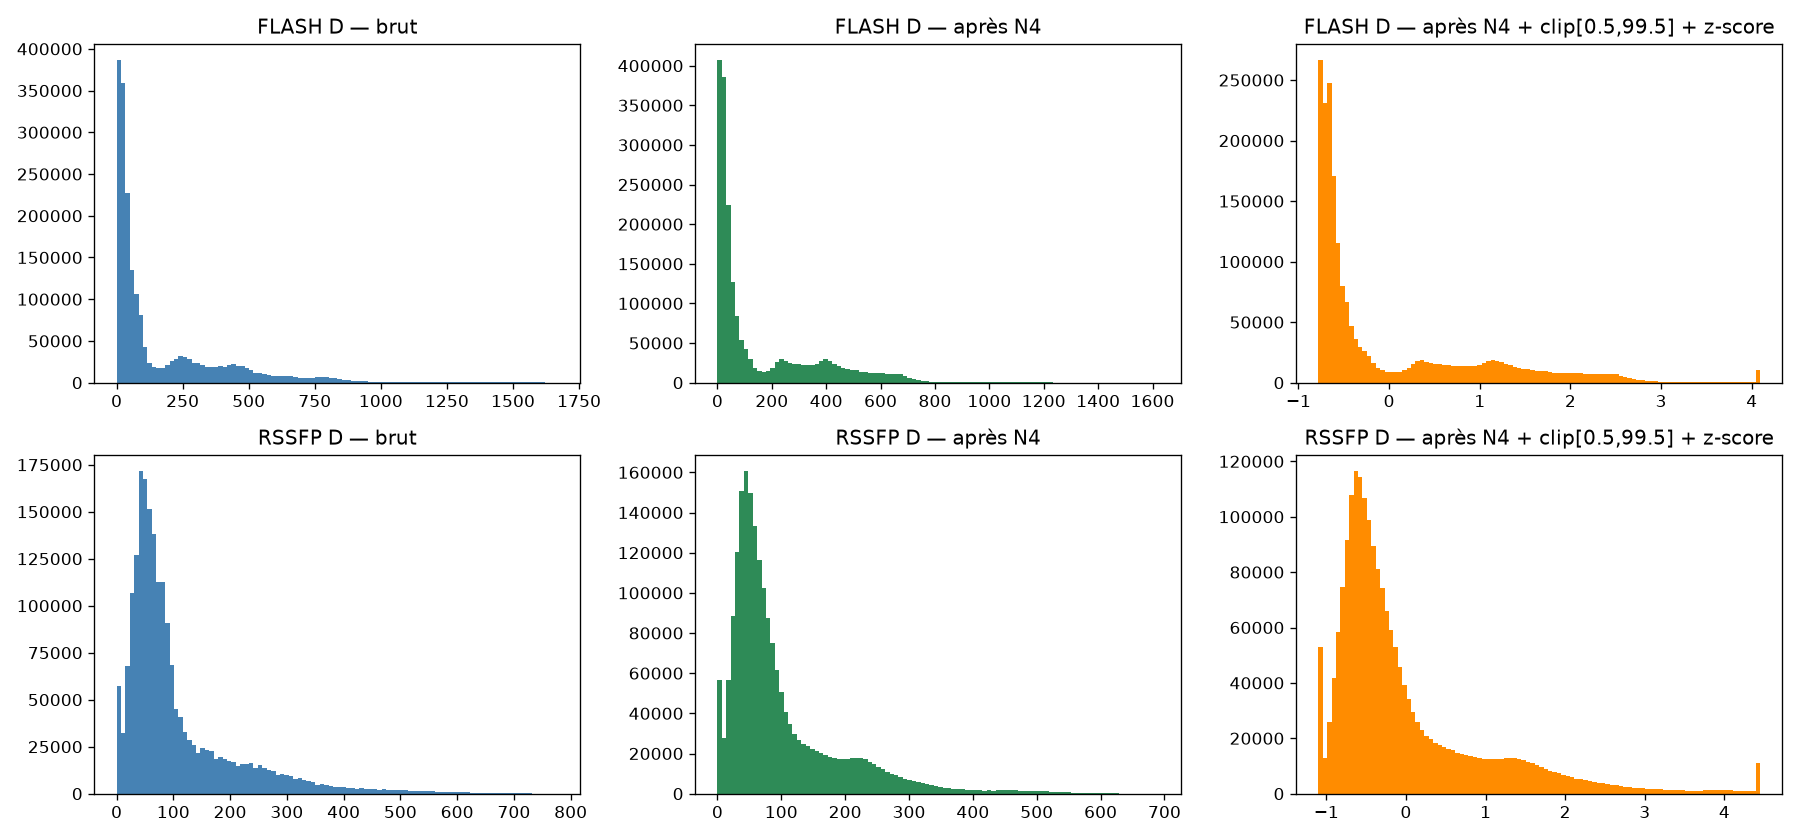
\includegraphics[width=\textwidth]{figures/validation_normalisation_hist.png}
\end{center}

Histogrammes d'intensité, FLASH D et RSSFP D du même patient, à chaque étape du
pipeline (brut / après N4 / après clip+z-score) --- la forme générale de la
distribution est préservée à chaque étape, seule l'échelle change, cohérent avec la
table de CNR ci-dessus.

\section{Résolution des structures par nom}

Reprend sans changement la logique validée en EDA (\S\ref{chap:exploration}) : chaque
structure est résolue par son nom d'en-tête (table d'alias \texttt{MCS}
$\to$ \texttt{MSC}, etc.), jamais par sa valeur de \texttt{LabelValue} brute --- l'EDA a
montré que PB est stockée sous 3 valeurs de label différentes (5, 6, 7) selon le
fichier.

\section{Exécution du pipeline complet}

\texttt{scripts/build\_dataset.py} exécuté sur les 56 séries :

\begin{itemize}[nosep]
    \item \textbf{51/56 séries traitées avec succès}, mêmes 5 exclues que dans l'EDA
        (géométrie non résolue).
    \item Temps de traitement : 0,3 à 1,3\,s par série (dominé par N4), quelques
        dizaines de secondes pour l'ensemble.
    \item Sortie : \texttt{DATA\_processed/<patient>/<série>/\{image.npy, label.npy\}}
        (image en \texttt{float32} normalisée, masque en \texttt{uint8} canonique
        1--6), $\approx$ 498\,Mo au total, plus un \texttt{manifest.csv} récapitulatif
        (statut, spacing d'origine, rééchantillonnage appliqué ou non, forme finale,
        temps de traitement).
    \item \texttt{2017-110\_01-0224-V1MR} (outlier de barycentre récurrent, \S
        \ref{sec:composantes-connexes}, jamais formellement vérifié sous 3D Slicer) est
        traitée normalement mais marquée \texttt{a\_verifier\_manuellement=True} dans
        le manifeste --- traçable sans bloquer le pipeline, en attendant la
        vérification.
\end{itemize}

\begin{center}
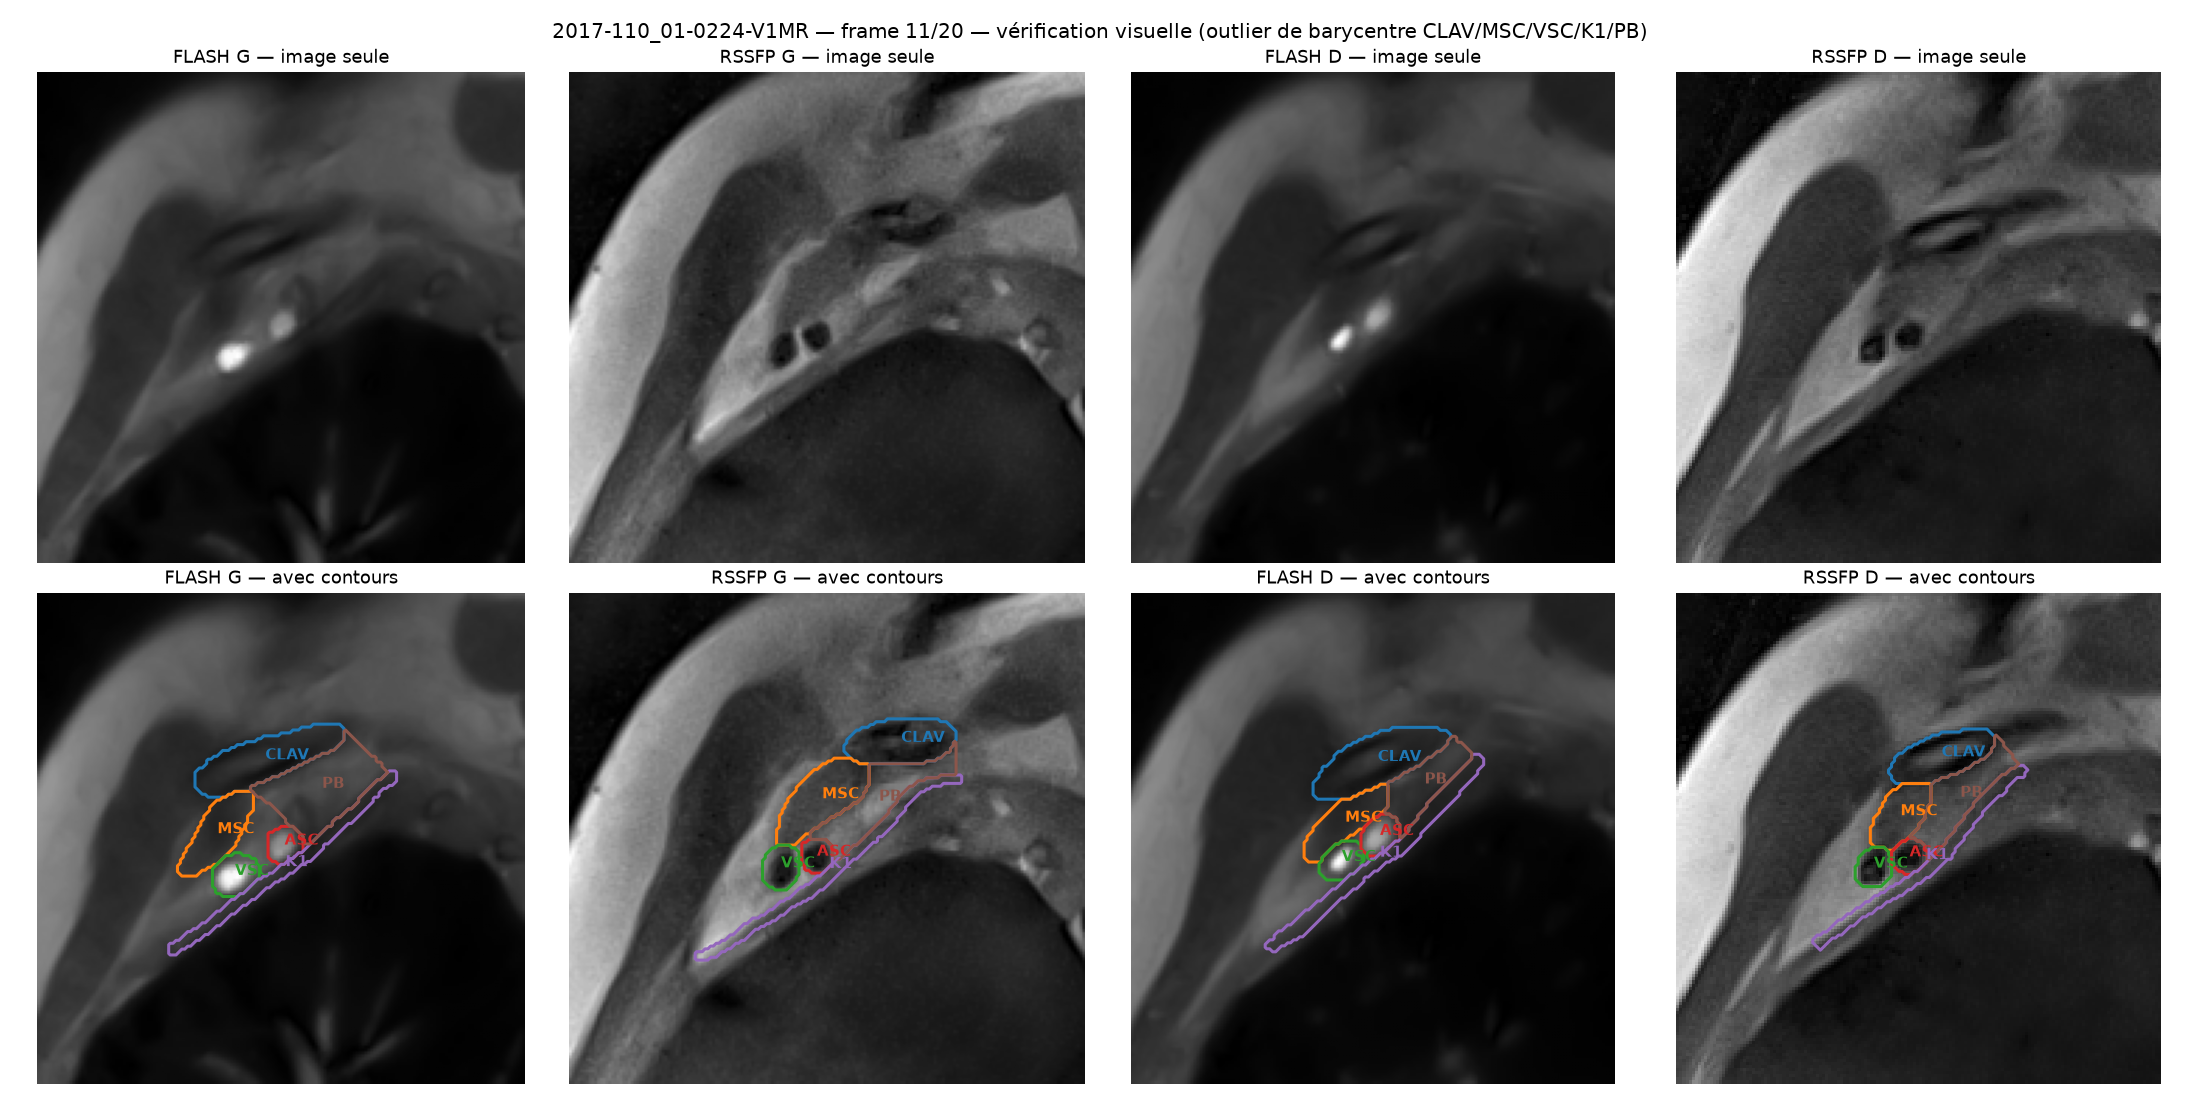
\includegraphics[width=\textwidth]{figures/verification_0224.png}
\end{center}

Vérification visuelle préliminaire (pas un substitut à 3D Slicer) sur ce patient : les
4 séries (FLASH/RSSFP D/G), une frame centrale, contours superposés. Rien ne saute aux
yeux comme clairement faux --- CLAV suit l'os incurvé, VSC/ASC sont bien positionnées
sur l'amas de vaisseaux, K1 trace une structure longue cohérente, et les 4 séries se
ressemblent entre elles. N'exclut pas une erreur subtile non visible sur cette seule
frame (1 sur 20) ; ne remplace pas la vérification manuelle complète sous 3D Slicer,
qui nécessite un jugement anatomique/clinique.

\section{Split train/val/test}

\subsection{Décision et bug de méthode corrigé}

Split au niveau \textbf{patient} (13 patients éligibles sur 14 --- \texttt{0222} est
entièrement exclu, 0 série utilisable), pour éviter toute fuite entre séries D/G ou
FLASH/RSSFP d'un même patient.

\textbf{Bug trouvé et corrigé pendant l'implémentation} : la première version du split
tirait les 13 patients éligibles au hasard sans distinguer ceux marqués
\texttt{a\_verifier\_manuellement} --- résultat, \texttt{2017-110\_01-0224-V1MR} est
tombé par hasard dans le split de \textbf{validation}. Risqué : si ses annotations
s'avèrent erronées lors de la vérification 3D Slicer, ça aurait faussé silencieusement
les métriques d'évaluation, pas seulement l'entraînement. \textbf{Corrigé} : tout
patient marqué \texttt{a\_verifier\_manuellement} est désormais forcé en train (impact
dilué sur beaucoup de cas) et ne peut jamais tomber en val/test tant qu'il n'est pas
confirmé.

\textbf{Justification (littérature)} : Varoquaux \& Cheplygina (2022, \emph{npj Digital
Medicine}, ``Machine learning for medical imaging: methodological failures and
recommendations'') identifient la fuite de données au niveau patient et l'absence de
curation des cas atypiques avant entraînement comme deux des causes les plus
fréquentes de sur-estimation de performance en imagerie médicale --- les deux
préoccupations traitées ici.

\subsection{Résultat (graine 42)}

\begin{center}
\begin{tabular}{ll}
\toprule
Split & Patients \\
\midrule
Train (9) & 0224, 0226, 0227, 0228, 0229, 0230, 0236, 0237, 0241 \\
Val (2)   & 0223, 0231 \\
Test (2)  & 0240, 0242 \\
\bottomrule
\end{tabular}
\end{center}

(\texttt{2017-110\_01-0222-V1MR} exclu, 0 série utilisable ; identifiants patient
abrégés au numéro final.)

\subsection{Point résolu en Phase 1}

Avec seulement 13 patients éligibles, un split fixe laisse très peu de patients en
val/test (2 chacun) --- l'évaluation sur un split aussi petit serait bruitée, une
variation d'un seul patient pouvant faire basculer une métrique de façon importante.
\textbf{Décision prise en Phase 1} (chapitre Protocole expérimental) : abandon du
split fixe au profit d'une validation croisée \texttt{KFold} au niveau patient
($k=3$) --- chaque patient passe exactement une fois en validation, et la comparaison
FLASH vs RSSFP est faite au niveau patient plutôt qu'au niveau fold pour rester
statistiquement exploitable malgré le petit $k$ (voir justification détaillée dans
le chapitre Protocole expérimental).

Reste ouvert, non tranché avec l'encadrant : si D et G doivent être traités comme un
flip horizontal l'un de l'autre --- en attendant, le flip horizontal n'est pas utilisé
comme augmentation (choix conservateur, voir chapitre Méthodologie).

\section{Sources et justifications --- récapitulatif}

\begin{center}
\begin{tabular}{lp{9cm}}
\toprule
Décision & Source \\
\midrule
Rééchantillonnage vers un spacing cible & nnU-Net, Isensee et al. (2021), \emph{Nature Methods} \\
Correction N4 & N4ITK, Tustison et al. (2010), \emph{IEEE TMI} --- justification spécifique au projet (interprétabilité), pas une reprise de la pratique nnU-Net par défaut \\
Z-score par cas (IRM) & nnU-Net (défaut confirmé dans la documentation officielle du dépôt) \\
Clip percentile avant z-score & Adaptation empirique motivée par l'EDA, pas un défaut nnU-Net \\
Histogram matching (écarté) & Nyúl \& Udupa (1999), \emph{Magnetic Resonance in Medicine} \\
Split patient-level, exclusion des cas non vérifiés & Varoquaux \& Cheplygina (2022), \emph{npj Digital Medicine} \\
\bottomrule
\end{tabular}
\end{center}

\todonote{Vérification manuelle encore en attente (non bloquante pour la Phase 1,
ces séries restent exclues) : les 6 séries non résolues
(\texttt{0222} $\times$4, \texttt{0223/FLASH D}, \texttt{0224} $\times$4).}


\chapter{Champ de ce chapitre}

À partir d'ici, ce document remplace l'approche de baseline suivie initialement
(grille d'ablation augmentation$\times$crop sur un modèle pooled, fold 0/1 --- non
reprise ici, voir historique git pour cette étape intermédiaire si besoin). Deux
différences de fond motivent ce changement d'approche :

\begin{itemize}[nosep]
    \item \textbf{Méthodologie décidée a priori, à partir de la littérature} --- pas
        par comparaison empirique de plusieurs configurations sur 2 folds (l'ancienne
        approche a montré ses limites : effets qui changent de signe entre folds sur
        un dataset de 13 patients, voir \S\ref{sec:limite-ancienne-approche}).
    \item \textbf{Deux modèles spécialisés par séquence} (FLASH, RSSFP) dès le
        départ, pas un modèle pooled suivi d'une comparaison a posteriori --- répond
        directement à la question clinique du projet (dynamique vs statique,
        FLASH vs RSSFP) sans détour.
\end{itemize}

\section{Ce qui est repris de l'exploration préliminaire}
\label{sec:limite-ancienne-approche}

Deux résultats de l'exploration initiale (chapitre~\ref{chap:exploration}) restent
valides et informent ce document, indépendamment de la méthodologie d'entraînement
retenue :

\begin{description}[style=nextline]
    \item[Bug d'alignement H/W] Le labelmap (\texttt{.seg.nrrd}) et l'image DICOM
        étaient transposés sur leurs deux premiers axes -- indétectable par une
        simple comparaison de \texttt{shape} (les deux axes valent 320) ou par le
        raisonnement géométrique a priori (les cosinus directeurs concordaient malgré
        tout). Confirmé empiriquement par un score de gradient de bord (les contours
        du masque doivent tomber sur de vrais bords d'intensité) : l'orientation
        transposée obtient un score $\sim$1,6--2$\times$ supérieur. Ce bug avait
        inversé la conclusion FLASH vs RSSFP sur le contraste (CNR) -- corrigé, FLASH
        montre un avantage CNR robuste au niveau population sur ASC/VSC
        (+1,84 et +2,31 vs écart-type inter-patient de 0,53 et 0,43).
    \item[Fragmentation structurelle de K1] L'analyse en composantes connexes de
        l'exploration a identifié K1 et MSC comme les structures les plus souvent
        fragmentées en plusieurs composantes dans la vérité terrain (K1 : 7/56
        séries). Cette observation, indépendante de tout choix d'entraînement, sert
        de grille de lecture pour les résultats de ce document : si K1 reste
        systématiquement la structure la plus faible ici aussi, ça confirme une
        difficulté structurelle plutôt qu'un artefact de méthodologie.
\end{description}

Les résultats d'entraînement de l'exploration préliminaire (grille aug$\times$crop,
folds 0/1 du modèle pooled) ne sont \textbf{pas} repris ici -- retirés du rapport
(disponibles dans l'historique git si besoin de les reconsulter), ce document part
d'une méthodologie déjà décidée, pas d'une comparaison empirique menant à cette
décision.

\chapter{Méthodologie}
\label{chap:methodologie}

Principe directeur : chaque choix est ancré dans la littérature \emph{avant}
l'entraînement, pas ajusté après coup par comparaison empirique sur un dataset trop
petit (13 patients) pour trancher des écarts fins de manière fiable.

\section{Fonction de perte}

\textbf{Dice + Cross-Entropy pondérée} (inchangé par rapport à l'exploration
préliminaire) --- Ma et al. (2021, \emph{Medical Image Analysis}, ``Loss odyssey'')
montrent que cette combinaison est la plus robuste sur 6 datasets/10+ centres,
particulièrement sur les tâches à déséquilibre de classe modéré, exactement le cas ici
(ratio 4,4$\times$ entre PB et ASC, EDA \S distribution de taille). Alternatives
considérées et écartées : Generalized Dice Loss (Sudre et al. 2017) et Unified Focal
Loss (Yeung et al. 2021), conçues pour un déséquilibre \emph{extrême} -- non
justifiées ici, et la pondération CE par fréquence inverse déjà en place
(\texttt{compute\_class\_weights}, mesurée empiriquement sur le train set) répond au
même besoin sans hyperparamètre supplémentaire à régler.

\section{Métriques}

\textbf{Dice + Hausdorff-95 + Normalized Surface Distance (NSD)} --- ajout du NSD par
rapport à l'exploration préliminaire. Justifié par Maier-Hein et al. (2024,
\emph{Nature Methods}, ``Metrics reloaded''), la référence de consensus international
sur le choix des métriques de segmentation : combiner une métrique de recouvrement
(Dice) avec des métriques de frontière (HD95 \emph{et} NSD) est recommandé
explicitement, ces métriques étant insuffisamment corrélées pour se substituer l'une
à l'autre. NSD calculé avec une tolérance $\tau=2$px (spacing rééchantillonné à 1mm
en Phase 0, donc $\approx$2mm) -- voir \texttt{src/metrics.py},
\texttt{nsd\_per\_class}. Toujours rapportées par structure, jamais macro-moyennées
(convention BraTS, déjà justifiée dans l'exploration préliminaire).

\section{Augmentation de données}

\textbf{Toujours activée, dès le premier entraînement -- pas testée en option.}
nnU-Net (Isensee et al. 2021, \emph{Nature Methods}), la référence du domaine,
applique l'augmentation par défaut sur \emph{toutes} les tâches, sans jamais la
traiter comme un choix à valider empiriquement au cas par cas. Paramètres repris de
l'exploration préliminaire (\texttt{src/augmentation.py}, \texttt{JointAugmentation})
: rotation $\pm12°$, scaling 0,9--1,1$\times$, déformation élastique légère
($\alpha=15$, $\sigma=4$, $p=0,3$), gamma/luminosité ($p=0,5$ chacun) --- délibérément
plus conservateurs que les défauts nnU-Net ($\pm30°$, 0,7--1,4$\times$), écart
\textbf{assumé et justifié} : la Phase 0 a déjà rééchantillonné toutes les séries à
un spacing physique commun, un scaling aussi agressif que nnU-Net réintroduirait la
variance d'échelle que ce rééchantillonnage visait à supprimer. Flip horizontal
toujours exclu (question D/G miroir anatomique non tranchée avec l'encadrant) ---
second écart assumé au défaut nnU-Net.

\section{Recadrage ROI (crop)}

\textbf{Non utilisé dans ce baseline.} Un crop fixe non appris (tel qu'exploré en
Phase 1 exploratoire) n'est pas une pratique standard -- la référence pour les petites
structures dans une grande image est le cascade coarse-to-fine à deux étages
(localisateur puis modèle fin, ex. Roth et al., Zhu et al. pour le pancréas, marge de
15px après localisation dans certaines implémentations), pas un crop fixe par
statistiques de population. nnU-Net lui-même ne fait pas de crop fixe par défaut.

\textbf{Limite assumée, à documenter honnêtement} : nnU-Net compense le déséquilibre
fond/structure non pas en ignorant le problème, mais par un échantillonnage de
patchs orienté premier-plan pendant l'entraînement (sur-échantillonnage des régions
contenant la structure cible). Ce pipeline n'a pas d'équivalent -- image entière,
échantillonnage uniforme des frames. Ne pas présenter l'absence de crop comme un
alignement complet sur nnU-Net ; c'est un choix de simplicité pour ce baseline,
documenté comme piste d'amélioration possible (cascade complet ou échantillonnage
pondéré), pas comme équivalent fonctionnel.

\section{Ordre d'implémentation retenu}

\begin{enumerate}[nosep]
    \item Métriques (ajout du NSD) -- nécessaire pour évaluer correctement tout run.
    \item Perte -- inchangée.
    \item Augmentation -- activée par défaut dès le premier entraînement de chaque
        modèle, jamais ajoutée après coup.
    \item Crop -- non implémenté dans ce baseline (voir limite ci-dessus).
\end{enumerate}

\chapter{Protocole expérimental}

\section{Deux modèles spécialisés, pas de modèle pooled}

Un modèle FLASH-only (séries \texttt{FLASH D/G} uniquement) et un modèle RSSFP-only
(séries \texttt{RSSFP D/G} uniquement), même architecture et hyperparamètres
(U-Net 2D, 4 niveaux, base\_ch=32, $\approx$7,7M paramètres --- inchangé de
l'exploration préliminaire). Pas de 3e modèle pooled : la question de recherche est
directement comparative (FLASH vs RSSFP), un modèle pooled n'y répond pas et
triplerait le travail des phases XAI suivantes sans bénéfice pour cette question.

\textbf{Compromis assumé} : chaque modèle spécialisé n'a accès qu'à la moitié des
données du modèle pooled (une seule paire D/G au lieu de deux) --- compromis
symétrique entre les deux modèles, donc la comparaison reste valide même si les Dice
absolus sont probablement inférieurs à un modèle pooled hypothétique.

\section{Validation croisée : k=3, appariement au niveau patient}
\label{sec:protocole-cv}

$k=3$ folds au niveau patient (\texttt{src/splitting.py}), réduit de $k=5$ dans
l'exploration préliminaire --- compromis coût de calcul / fiabilité pour 2 modèles au
lieu d'1.

\textbf{Point méthodologique important} : la comparaison finale FLASH vs RSSFP ne
repose \textbf{pas} sur une moyenne des 3 Dice de fold (ce qui donnerait seulement 3
paires, insuffisant pour un test statistique -- avec $n=3$, un test de Wilcoxon
signé-apparié ne peut atteindre $p<0{,}05$ quelle que soit l'ampleur de l'effet réel,
$p_{min} \approx 0{,}25$). Chaque patient passant exactement une fois en validation
par modèle sur l'ensemble des 3 folds, la comparaison est faite \textbf{au niveau
patient} ($n\approx13$ paires) : score du patient X sous le modèle FLASH vs score du
même patient X sous le modèle RSSFP. C'est la pratique établie en littérature de
segmentation médicale pour comparer deux méthodes (test de Wilcoxon signé-apparié sur
scores par cas, avec correction de Holm-Bonferroni pour les comparaisons multiples --
6 structures testées séparément). Implémenté dans
\texttt{scripts/train\_baseline.py}, \texttt{evaluate\_per\_patient} ---
chaque run ajoute ses lignes patient$\times$structure à
\texttt{report/figures/baseline\_per\_patient\_metrics.csv}, dédupliquées par
(patient, séquence, structure) pour éviter les doublons en cas de relance.

\section{Commande}

\begin{center}
\texttt{python scripts/train\_baseline.py --sequence \{FLASH,RSSFP\} --fold \{0,1,2\}
--epochs 30}
\end{center}

6 runs au total (2 séquences $\times$ 3 folds).

\chapter{Résultats}
\label{chap:resultats}

\todonote{5 runs restants (FLASH fold 1--2, RSSFP fold 0--2) avant de pouvoir faire
la comparaison statistique appariée par patient (\S\ref{sec:protocole-cv}). Cette
section sera complétée à chaque run.}

\section{FLASH, fold 0}

30 epochs, 9 patients train (360 frames) / 4 patients val (140 frames ---
\texttt{2017-110 01-0229-V1MR}, \texttt{\_0223}, \texttt{\_0226}, \texttt{\_0227}).
Meilleur checkpoint à l'epoch 26 (Dice moyen structures, moyenné par patient puis par
structure = 0,7046).

\begin{center}
\begin{tabular}{lrrrrr}
\toprule
Structure & Dice & Précision & Rappel & Hausdorff-95 (px) & NSD \\
\midrule
CLAV & 0,8199 & 0,7659 & 0,8919 & 4,50 & 0,8709 \\
MSC  & 0,7231 & 0,6399 & 0,8511 & 4,60 & 0,8204 \\
VSC  & 0,8043 & 0,7741 & 0,8477 & 4,65 & 0,8863 \\
ASC  & 0,6728 & 0,6229 & 0,7560 & 6,65 & 0,7956 \\
K1   & 0,4812 & 0,3711 & 0,7377 & 13,76 & 0,6453 \\
PB   & 0,6944 & 0,6747 & 0,7619 & 8,93 & 0,6935 \\
\bottomrule
\end{tabular}
\end{center}

\begin{center}
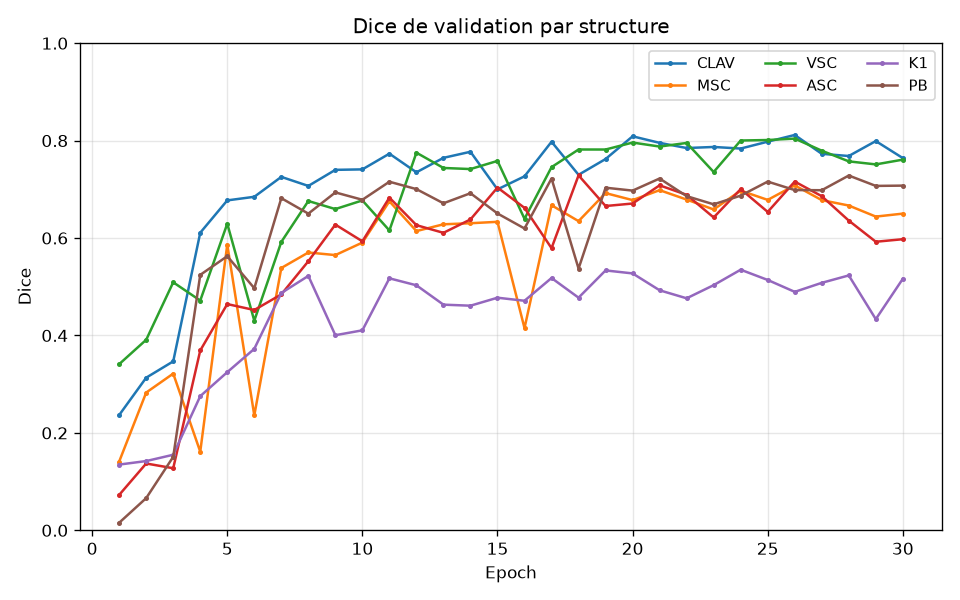
\includegraphics[width=0.75\textwidth]{figures/baseline_FLASH_fold0_dice_curve.png}
\end{center}

\textbf{K1 confirmé comme structure la plus faible} (Dice 0,48, HD95 13,76px, NSD
0,65 -- le NSD le plus bas des 6 structures) --- cohérent avec la fragmentation
structurelle documentée en exploration préliminaire (\S\ref{sec:limite-ancienne-approche})
et avec les résultats du modèle pooled (exploration préliminaire, non repris ici en
détail) : troisième configuration d'entraînement indépendante où K1 ressort en
dernier, ce qui renforce l'hypothèse d'une difficulté structurelle plutôt que d'un
artefact de méthodologie ou de split.

\textbf{ASC plus bas que dans le modèle pooled} (0,67 ici contre $\sim$0,75--0,80
dans l'exploration préliminaire) --- cohérent avec le compromis assumé
(\S\ref{chap:resultats}, moitié des données pour un modèle spécialisé) : à confirmer
si ce n'est pas simplement un effet de ce fold particulier, sur les folds 1--2.

\textbf{Anomalie de timing, présente mais atténuée} : epochs 20, 22, 24 ont pris
250--455s contre $\approx$80--130s pour les autres -- nettement moins sévère que les
runs de 12--13h observés sur ``sans aug + crop'' dans l'exploration préliminaire
(qui ont motivé la décision de retirer le crop de ce baseline), mais pas totalement
absente. Le crop n'était donc pas l'unique cause -- à surveiller sur les 5 runs
restants avant de conclure quoi que ce soit sur l'origine exacte.

\chapter{Analyse statistique}

\todonote{À faire une fois les 6 runs terminés : test de Wilcoxon signé-apparié par
structure (FLASH vs RSSFP, $n\approx13$ patients), correction de Holm-Bonferroni pour
les 6 tests (6 structures), et rapport des tailles d'effet (pas seulement les
p-values) -- voir \S\ref{sec:protocole-cv} pour la justification du choix
méthodologique de ce test.}

\end{document}
